\chapter{Supersymmetry \& Grand Unification: Lecture 1}

These notes follow Leonard Susskind's opening lecture in the supplementary course on supersymmetry and grand unification, curated by LazyingArt LLC. The lecture begins one step earlier than supersymmetry itself. It begins with renormalization: first as a way of throwing away microscopic detail that does not matter for the question at hand, and then as a way of estimating what the discarded short-distance physics must do to the parameters we measure. We will keep that order. The chapter therefore unfolds as the lecture unfolds: coarse-graining, then dimensional analysis, then scalar mass renormalization, then the Higgs hierarchy problem, then the much better behavior of fermions, and finally vacuum energy.

\section{Renormalization as Coarse-Graining}

Susskind opens the course by saying that many of the ideas to come grew out of puzzles in the renormalization of the Standard Model. But he does not begin with counterterms, regularization schemes, or formal perturbation theory. Instead he asks us to remember that physics repeatedly changes its effective language as the scale of interest changes.

\begin{definition}
In the sense emphasized throughout this lecture, renormalization has two ingredients:
\begin{enumerate}
\item we eliminate from the description degrees of freedom associated with distances too small, or motions too fast, to matter for the problem we are actually asking;
\item we replace their net effect by effective parameters in a coarser description.
\end{enumerate}
The second half of the subject is dimensional analysis: once the short-distance modes are identified, dimensional analysis often tells us how large their effects must be.
\end{definition}

The lecture then climbs, deliberately and patiently, through a ladder of effective descriptions. If we are doing nuclear physics, we may begin with quarks, because quarks are the microscopic constituents. But once we have extracted the masses, spins, and interactions of protons and neutrons, we are free to describe the nucleus as a nonrelativistic many-body system built from those slower composite objects. If we move up to atomic physics, we need even less microscopic information. The detailed structure of the nucleus mostly drops out; its mass and charge are the main data that survive. Once we know those, we start over again and treat nuclei and electrons as the relevant elementary ingredients.

The same step is taken yet again when we go from atoms to molecules. At each stage we solve just enough of the finer theory to determine the parameters that matter at the next scale, and then we forget how those parameters were produced. The description becomes less microscopic, but more useful. That is the sense in which renormalization is already part of ordinary physics long before we apply the word to quantum field theory.

\section{Molecules as the Prototype Example}

The lecture's first real mathematical example is a pair of atoms, reimagined as two heavy nuclei together with their electrons. The aim is to replace the detailed electronic cloud by an effective force between two slow, heavy objects. Susskind's motivation is physical before it is formal: we would like to describe atoms as particles with forces between them, not as bowling balls permanently accompanied by a swarm of tiny fast flies.

Because relativity is irrelevant at molecular scales, he starts from nonrelativistic quantum mechanics. A cleaned reconstruction of the Hamiltonian written on the board is
\begin{equation}
H=
\frac{P_1^2}{2M}
+\frac{P_2^2}{2M}
+\frac{e^2}{R_{12}}
+\sum_i \frac{q_i^2}{2m}
+\sum_{i<j}\frac{e^2}{r_{ij}}
-\sum_i\left(\frac{e^2}{R_{1i}}+\frac{e^2}{R_{2i}}\right).
\end{equation}
Here \(P_1,P_2\) are the nuclear momenta, \(M\) is the nuclear mass, \(q_i\) are the electron momenta, \(m\) is the electron mass, \(R_{12}\) is the distance between the nuclei, \(r_{ij}\) is the separation of two electrons, and \(R_{1i},R_{2i}\) are the distances from the \(i\)-th electron to the two nuclei.

\begin{remark}
The board image fixes the structure of the Hamiltonian more securely than it fixes every symbol. In particular, the electron momentum notation and the electron-nucleus attraction terms are partly obscured in the frame. The formula above is therefore a cautious transcript-backed reconstruction rather than a literal blackboard transcription.
\end{remark}

\begin{figure}[htbp]
\centering

\includegraphics[width=0.78\textwidth]{lecture_01_figure_02.png}
\caption{Molecular Hamiltonian with the electron sector visually grouped as a subproblem.}
\end{figure}

What matters next is the separation of time scales. The nuclei are heavy. The electrons move much more rapidly. Susskind's picture is that the nuclei move so slowly that, in first approximation, we may nail them down and solve only for the electronic motion in that fixed nuclear background. We group all electron-dependent terms together and treat them as the Hamiltonian of the electrons alone, with \(R_1\) and \(R_2\) held fixed.

We then solve the electronic Schr\"odinger problem and keep the lowest eigenvalue,
\begin{equation}
E_{\mathrm{el}}=E_{\mathrm{el}}(R_1,R_2).
\end{equation}
This is the ground-state energy of the electrons in the background of stationary nuclei. Since it depends only on the nuclear positions, it can be absorbed into an effective potential for the nuclei:
\begin{equation}
V_{\mathrm{eff}}(R_1,R_2)=\frac{e^2}{R_{12}}+E_{\mathrm{el}}(R_1,R_2).
\end{equation}

The lecture emphasizes the qualitative shape. At very short separation the Coulomb repulsion of the nuclei dominates, so the potential is strongly repulsive. At very large separation the interaction becomes weak. Between the two there is an attractive region due to the electrons. Once that effective potential has been found, we no longer track the electronic cloud explicitly. The fast microscopic degrees of freedom have been eliminated and replaced by a renormalized Hamiltonian for the slow ones.

That is the prototype. Susskind explicitly pauses here to say that this, too, is renormalization.

\section{From Effective Potentials to Field Theory}

Only after the molecular example has done its work does the lecture pivot to field theory. The transition is exact: in quantum field theory the modes we wish to eliminate are the very short-wavelength, very high-frequency, very high-energy ones. Small usually goes with fast. The ultraviolet modes are the field-theory analog of the fast electrons in the molecular problem.

Before launching into diagrams, however, Susskind deliberately interrupts the story and inserts a small toolkit. ``Before we do that,'' he says in effect, ``let us do some dimensional analysis.'' This is not a digression. It is what will allow the loop estimates to be read off rather than computed in detail.

Setting \(c=\hbar=1\), one independent dimension remains. We may take it to be length. Then
\begin{equation}
[M]=[E]=[p]=L^{-1},
\qquad
[x]=[t]=L.
\end{equation}
So mass, energy, and momentum all count as inverse length, while space and time count as length. Once this is fixed, the size of propagators and couplings becomes almost forced upon us.

\section{Scalar Fields, Propagators, and Mass Renormalization}

The lecture now chooses the cleanest possible setting: one scalar field \(\phi\). On the board the theory is introduced schematically by first writing the local Lagrangian density,
\begin{equation}
\mathcal{L}=(\partial_\mu\phi)^2-V(\phi),
\end{equation}
and then, on the next line, the action,
\begin{equation}
S=\int d^4x\,\mathcal{L}.
\end{equation}

\begin{figure}[htbp]
\centering

\includegraphics[width=0.78\textwidth]{lecture_01_figure_03.png}
\caption{The lecture's two-step move from local Lagrangian density to spacetime action.}
\end{figure}

\begin{remark}
The board writes the scalar theory in a deliberately schematic normalization. We keep that form rather than silently inserting textbook factors of \(1/2\).
\end{remark}

Because \(\hbar=1\), the action is dimensionless. Therefore the Lagrangian density must have dimensions \(L^{-4}\). The kinetic term then fixes the dimension of the field itself:
\begin{align}
[S]&=1,
&
S&=\int d^4x\,\mathcal{L},
\\
[\mathcal{L}]&=L^{-4},
&
[(\partial_\mu\phi)^2]&=L^{-4}.
\end{align}
Since \([\partial_\mu]=L^{-1}\), we obtain
\begin{equation}
[\phi]^2L^{-2}=L^{-4}
\qquad\Longrightarrow\qquad
[\phi]=L^{-1}.
\end{equation}
This is exactly the kind of elementary dimensional fact that the lecture wants us to keep in our pocket.

Next the potential is expanded:
\begin{equation}
V(\phi)=\frac{m^2}{2}\phi^2+g\phi^3+\lambda\phi^4+\cdots.
\end{equation}
Since \(V\) must also have dimensions \(L^{-4}\), we read off
\begin{equation}
[g]=L^{-1},
\qquad
[\lambda]=1.
\end{equation}
The point is immediate. The coefficients in the potential become the coefficients of Feynman vertices. The cubic term gives a three-point vertex weighted by \(g\). The quartic term gives a four-point vertex weighted by \(\lambda\). The quadratic term gives a two-point insertion: the lecture draws it as a particle that comes in, is absorbed, and is emitted again from essentially the same point.

The second ingredient is the propagator. Susskind defines it operationally before he defines it algebraically. It is the amplitude to create a particle at one spacetime point and detect it at another. In the lecture this is written as
\begin{equation}
\langle 0|\phi(y)\phi(x)|0\rangle.
\end{equation}
Now the vacuum has no dimensions, but each \(\phi\) has dimensions \(L^{-1}\), so the whole object has dimensions \(L^{-2}\). If the scalar is massless, there is no intrinsic length scale in the problem except the separation of the two points themselves. Therefore the propagator must scale schematically as
\begin{equation}
\langle 0|\phi(y)\phi(x)|0\rangle \propto \frac{1}{(x-y)^2}.
\end{equation}
Here one should read \((x-y)^2\) schematically as the Lorentz-invariant squared separation. The lecture is not deriving a fully normalized Green's function. It is isolating the short-distance behavior. And that behavior is what matters: the propagator blows up as the points approach one another. That is the source of ultraviolet divergence.

Now the lecture asks what the mass term really means in an effective theory. At the microscopic level the bare \(m^2\phi^2/2\) term is the simplest local two-point insertion. But if our experimental microscope cannot resolve distances smaller than some cutoff \(\delta\), then any short-distance process that imitates a particle coming in and going out again from essentially the same place must be counted as part of the mass term. This is where renormalization enters.

The first example uses the quartic coupling. A particle comes in, goes out, and at the same point a short virtual line is emitted and reabsorbed. If the separation is smeared only over distances of order \(\delta\), the propagator contributes \(1/\delta^2\), so
\begin{equation}
\delta m^2\sim \frac{\lambda}{\delta^2}.
\end{equation}
The next example is a higher-order diagram with two quartic vertices. Here we must integrate over the relative separation of the two nearby points. To keep the notation straight, let \(\Delta^\mu\) denote the integration variable, while \(\delta\) denotes the cutoff distance. Then the lecture's dimensional estimate is
\begin{equation}
\lambda^2\int d^4\Delta\,\frac{1}{\Delta^6}\sim \frac{\lambda^2}{\delta^2}.
\end{equation}
The logic is simple: three propagators give \(\Delta^{-6}\), the four-dimensional measure gives \(d^4\Delta\), and the answer can depend only on the lower cutoff \(\delta\). So it must again scale like \(\delta^{-2}\).

The cubic interaction gives something slightly subtler. Two cubic vertices and two propagators produce
\begin{equation}
g^2\int d^4\Delta\,\frac{1}{\Delta^4}\sim g^2\log(\delta\,\mu_{\mathrm{ref}}),
\end{equation}
with a reference scale \(\mu_{\mathrm{ref}}\) inserted only to make the logarithm dimensionless. The lecture treats such logarithms cautiously and loosely; what matters for the present discussion is that logarithms are much weaker than power divergences. When \(\delta\) is very small, \(\delta^{-2}\) dominates \(\log\delta\).

Putting the structure together, we are led to the schematic relation
\begin{equation}
m_{\mathrm{phys}}^2\sim
m_0^2
+\frac{c_1\lambda}{\delta^2}
+\frac{c_2\lambda^2}{\delta^2}
+c_3 g^2\log(\delta\,\mu_{\mathrm{ref}})
+\cdots.
\end{equation}
The numerical coefficients and signs are not tracked in the lecture; the dominant message is that the scalar mass receives an infinite series of ultraviolet-sensitive corrections. And the same is true of the other couplings. The coefficient \(\lambda\) itself is renormalized by four-point diagrams, typically logarithmically, although Susskind stops short of turning that into a full study of beta functions.

\subsection{Question \& Answer}

\paragraph{Question.} What are we actually measuring: the input parameter or the renormalized one?

\paragraph{Answer.} We measure the renormalized one. The point of the cutoff description is precisely that we refuse to resolve all of the very short-distance structure. Once we do that, every unresolved process that imitates a local two-point interaction is lumped into the coefficient we call the mass term. The laboratory therefore does not see the pristine \(m_0^2\). It sees the effective coefficient after all the short-distance fluctuations we have chosen not to resolve have been summed into it.

\section{From Scalar Renormalization to the Higgs Hierarchy Problem}

At this point the lecture turns the scalar example into a crisis. For a scalar particle the additive corrections are present even if the bare mass vanishes. That is what makes the Higgs field dangerous. The lecture therefore asks us to recall the Higgs potential in its broken-symmetry form:
\begin{equation}
V(\phi)=-\frac{\mu^2}{2}\phi^2+\lambda\phi^4.
\end{equation}
Because the board normalization is schematic, the minimum is quoted in the lecture in the convention used there as
\begin{equation}
\phi_{\min}^2=f^2=\frac{\mu^2}{\lambda}.
\end{equation}
The key point is the scale, not the harmless convention-dependent factors. The vacuum expectation value is already known from electroweak physics:
\begin{equation}
f\sim 200\,\mathrm{GeV}.
\end{equation}
So unless \(\lambda\) is made implausibly tiny or huge, \(\mu\) is also of electroweak order.

Now compare that with the ultraviolet-sensitive scalar corrections. If we trust quantum field theory all the way down to a scale as short as the Planck length, then in GeV units the lecture estimates
\begin{equation}
\frac{1}{\delta^2}\sim 10^{38}\,\mathrm{GeV}^2.
\end{equation}
This is the point where the tone of the lecture changes. The scalar story is no longer just a technical example of renormalization. It becomes bad behavior. We want a Higgs parameter of electroweak size, but the short-distance contributions are incomparably larger. The precise number of decimal places shifts a bit in the spoken lecture, and the signs of the various contributions are left untracked, but the central point is stable: a huge collection of ultraviolet contributions must cancel to extraordinary precision in order to leave behind a weak-scale mass parameter.

That is the hierarchy problem, or fine-tuning problem, of the Higgs sector. It is not just that the weak scale is small compared with the Planck scale. It is that, in a scalar theory, the small physical parameter appears as the residue of a delicate cancellation among individually huge pieces.

\subsection{Question \& Answer}

\paragraph{Question.} Must the bare mass term cancel all the short-distance corrections?

\paragraph{Answer.} If we insist on keeping a very short-distance cutoff while also insisting that the physical Higgs parameter remain at the electroweak scale, then yes: the bare term must conspire with the radiative corrections so that the large ultraviolet-sensitive pieces almost exactly cancel. That is what the lecture means by fine-tuning. The problem is not that a correction exists. The problem is that a very small measured answer seems to require a cancellation among many much larger terms.

\section{Why Fermions Behave Better}

The lecture then deliberately changes tempo and asks the obvious question: if scalar masses are so unstable, why is the electron not equally disastrous? The answer comes from the structure of the fermion mass term,
\begin{equation}
m\bar{\psi}\psi.
\end{equation}
This term is linear in the fermion mass, not quadratic. More importantly, it flips chirality. It takes a left-chiral fermion into a right-chiral one, or vice versa. Susskind sometimes phrases this in helicity language in the lecture, but the mathematically safer language here is chirality.

\begin{figure}[htbp]
\centering

\includegraphics[width=0.78\textwidth]{lecture_01_figure_04.png}
\caption{The fermion mass term on the board, together with the lecture's chirality mnemonics.}
\end{figure}

The lecture now contrasts three kinds of vertices. Gauge-boson emission preserves chirality: \(L\to L\) and \(R\to R\). Scalar emission flips chirality: \(L\leftrightarrow R\). The mass insertion \(m\bar{\psi}\psi\) also flips chirality. The right-hand chalk sketches are mnemonic rather than literal Feynman graphs, but the underlying logic can be summarized schematically as follows.

\begin{figure}[htbp]
\centering
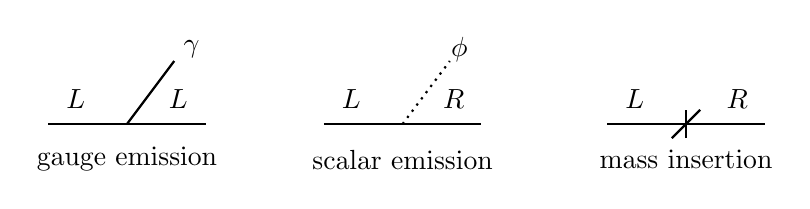
\begin{tikzpicture}[scale=1.0]
\draw[thick] (0,0)--(2,0);
\draw[thick] (1,0)--(1.6,0.8);
\node at (0.35,0.32) {$L$};
\node at (1.65,0.32) {$L$};
\node at (1.82,0.95) {$\gamma$};
\node at (1,-0.45) {gauge emission};

\draw[thick] (3.5,0)--(5.5,0);
\draw[dotted,thick] (4.5,0)--(5.1,0.8);
\node at (3.85,0.32) {$L$};
\node at (5.15,0.32) {$R$};
\node at (5.22,0.95) {$\phi$};
\node at (4.5,-0.45) {scalar emission};

\draw[thick] (7.1,0)--(9.1,0);
\draw[thick] (8.1,-0.18)--(8.1,0.18);
\draw[thick] (7.92,-0.18)--(8.28,0.18);
\node at (7.45,0.32) {$L$};
\node at (8.75,0.32) {$R$};
\node at (8.1,-0.45) {mass insertion};
\end{tikzpicture}
\caption{Schematic chirality mnemonics: gauge emission preserves chirality, while scalar emission and mass insertion flip it.}
\end{figure}

Now suppose the electron begins massless. Can photon emission and reabsorption generate a mass? No. Every gauge interaction preserves chirality, so no chain of such processes can turn left into right. Can scalar emission and reabsorption do it? Again no. A scalar emission flips chirality, but the corresponding reabsorption flips it back. Since the emitted scalar must be reabsorbed, the total number of scalar vertices is even, and the net effect cannot be a left-right transition. So neither gauge-boson loops nor scalar loops generate an additive fermion mass from zero.

To get a correction to the fermion mass, one must already insert a mass somewhere in the diagram. Then the correction is proportional to the starting mass itself. That is the lecture's crucial point. Schematically,
\begin{equation}
m_e=m_0+O(e^2m_0)+O(e^4m_0)+\cdots.
\end{equation}
Therefore if \(m_0=0\), the electron stays massless. If \(m_0\) is small, all the corrections remain small. One may still ask why the electron mass is numerically small compared with some deeper scale, but one is not forced into the same kind of catastrophic cancellation that afflicted the scalar.

\begin{remark}
The lecture slides back and forth between chirality and helicity in a physically intuitive way. For the purpose of writing the argument cleanly, chirality is the better variable. In the relativistic limit the lecture's helicity-based intuition remains a useful picture.
\end{remark}

Gauge bosons behave in the same protected way for the purpose at hand: if they begin massless, they remain massless to all orders. That is why the lecture insists that the Standard Model does not contain a separate fine-tuning problem for every light particle. The truly severe fine-tuning is the one tied to the Higgs field. If that one is solved, the rest of the light spectrum falls into place.

\subsection{Question \& Answer}

\paragraph{Question.} Why doesn't the electron have the same fine-tuning problem?

\paragraph{Answer.} Because the electron mass is protected against additive renormalization. Starting from zero, neither gauge interactions nor scalar emission-and-reabsorption can generate the chirality-flipping two-point structure that defines a fermion mass. Any nonzero correction already contains one explicit mass insertion, and is therefore proportional to the original mass itself. A small fermion mass may remain a fact in need of explanation, but it is not produced by canceling huge ultraviolet contributions against each other.

\section{Vacuum Energy and the Supersymmetry Outlook}

The lecture closes by widening the frame once more. There is another quantity that renormalization shifts: the energy of the vacuum itself. At first one is tempted to say, with Susskind, ``who cares?'' In ordinary nongravitational physics only energy differences matter. If the vacuum energy is shifted by a constant amount, that seems irrelevant so long as adding a particle adds the right extra amount of energy.

But gravity does care. Empty space gravitates if it carries energy. So the renormalization of the vacuum energy becomes physically significant once the gravitational field is allowed to respond to it.

In \(\phi^4\) theory the simplest vacuum-to-vacuum diagram contains no external particles. It consists only of a quartic vertex together with short propagators that begin and end within the unresolved region. The lecture's estimate is then
\begin{equation}
\delta\rho_{\mathrm{vac}}\sim \frac{\lambda}{\delta^4}.
\end{equation}
More complicated vacuum diagrams typically preserve the same \(\delta^{-4}\) behavior in this schematic discussion. So vacuum energy is also highly sensitive to short-distance physics.

The lecture therefore ends with two fine-tuning problems, not one. The Higgs mass is one. The vacuum energy is the other, and it is even more severe once gravity is included. Supersymmetry is introduced as a possible response to the first of these. It is not presented here as a cure for the cosmological-constant problem.

\subsection{Question \& Answer}

\paragraph{Question.} Does the fine-tuning depend on the arbitrary cutoff \(\delta\)?

\paragraph{Answer.} The contribution does depend on how far down in distance we trust the theory, but that is not an empty arbitrariness. We choose \(\delta\) to be the shortest scale at which we still believe the present quantum field theory makes sense. Then the accumulated contribution from all scales above that point is already there and must be accounted for. In that sense the estimate is a lower bound on the size of the problem. If the theory remains valid to even shorter distances, the scalar fine-tuning can only become worse. The lecture mentions scales as small as unification, around \(10^{16}\,\mathrm{GeV}\), as a conservative benchmark, with the Planck scale making the tension sharper still.

Two late clarifications from the lecture belong here. First, a scalar particle is a spin-zero particle; the Higgs is the central example in this discussion. Gauge bosons, by contrast, are spin-one particles. Second, although the simplest fermion and boson vacuum diagrams come with opposite signs, cancellation is not automatic. To cancel the vacuum energy naturally, masses and couplings would have to be matched with extraordinary precision. That is the kind of matching supersymmetry tries to impose in the Higgs sector, which is why it arrives here as the next subject of the course.

\section{Summary}

The lecture begins by teaching us how to think about renormalization before teaching us how to compute with it. We first integrate out fast electrons in a molecular problem and replace them by an effective potential for slow nuclei. We then carry the same idea into quantum field theory, where short-distance modes renormalize the coefficients in the Lagrangian. Dimensional analysis shows why scalar propagators are singular at short distance and why scalar mass terms are especially vulnerable to large additive corrections. That lesson becomes the Higgs hierarchy problem once the cutoff is taken seriously. Fermions and gauge bosons behave better because their masses are protected when they start from zero. Finally the lecture widens from the Higgs problem to the renormalization of vacuum energy, and ends by presenting supersymmetry not as a finished solution, but as the natural next attempt to tame the Higgs-sector fine-tuning.